\section{Predication}
\label{sec:predication}

For the reasons outlined in Section \ref{sec:costo_of_branch_prediction}, we can conclude that branches are expensive. Even when using state of the art branch predictors, certain branches are systematically hard to predict or have such low occurrences that not enough data are collected to perform a good prediction \cite{lin2019branch}. 
Predication is used to replace conditional branches with other instructions. In \textit{LLVM} and in \textit{GCC}, this is usually done during the backend optimization phase where the compiler works on the machine level representation of the code. The name that is generally given to this code optimization pass is \texttt{if-conversion}.

\begin{figure}[h!]
\centering
\begin{tabular}{ c c c }
\adjustbox{valign=m}{%
\begin{lstlisting}[language=C++, basicstyle=\ttfamily\small]
if (x > 0) y = 10;
else       y = 20;
\end{lstlisting}
}
&
\begin{tikzpicture}
    \draw[->, line width=0.5pt] (0,0) -- (1.5,0);
\end{tikzpicture}
&
\adjustbox{valign=m}{%
\begin{lstlisting}[language=C++, basicstyle=\ttfamily\small]
y = (x > 0)  * 10 + 
    (x <= 0) * 20;
\end{lstlisting}
}
\end{tabular}
\caption{Replacing a conditional branch with arithmetic operations.}
\label{fig:branching_predication_example}
\end{figure}

An example of this is presented in Figure \ref{fig:branching_predication_example} where code containing a conditional branch is replaced with code that performs exactly the same operation without the use of conditional branches. The example presented uses arithmetic properties to replace the branch and is usually referred to as \textbf{Arithmetic Predication} or \textbf{Branchless Programming}. Using Arithmetic Predication to replace branches presents limitations: multiplications are also expensive, and it's difficult to apply most of the time.

One way to overcome these limitations is by utilizing predicated instructions supported by the architecture, when these are available.
A predicated instruction in \armvs is an instruction which attaches conditions directly to instructions, allowing them to either execute or skip based on the condition's outcome.

\noindent\begin{minipage}{.45\textwidth}
\begin{lstlisting}[caption=Standard MOV in ARMv7 assembly, style=AsmStyle]{Name}
MOV R0, R1
\end{lstlisting}
\label{lst:add}
\end{minipage}\hfill
\begin{minipage}{.45\textwidth}
\begin{lstlisting}[caption=Predicated MOV in ARMv7 assembly,style=AsmStyle]{Name}
MOVGT R0, R1
\end{lstlisting}
\label{lst:cadd}
\end{minipage}

The \armvs architecture supports several predicated instructions. For example, the standard \texttt{MOV} instructions in Listing \ref{lst:add} takes the value in \texttt{R1} and moves it into \texttt{R0} while, the predicated version, \texttt{MOVGT}, showed in Listing \ref{lst:cadd} moves the value in \texttt{R1} to \texttt{R0} only when the last comparison was "greater than". \\

\begin{figure}[h!]
\centering
\begin{tabular}{ c c c c }
\adjustbox{valign=m}{%
\begin{lstlisting}[language=C++, basicstyle=\ttfamily\small]
if (x > 0) y = 10;
else y = 20;
\end{lstlisting}
}
&
\adjustbox{valign=m}{%
\begin{tikzpicture}
    \draw[->, line width=0.5pt] (0,0.5) -- (2, 1.5);
    \draw[->, line width=0.5pt] (0,-0.5) -- (2, -1.5);
\end{tikzpicture}
}
&
\adjustbox{valign=m}{%
\begin{minipage}{0.4\textwidth}
\textbf{Without Predication:}
\begin{lstlisting}[basicstyle=\ttfamily\small]
    cmp r0, #0
    bgt greater
    mov r1, #20
    b end
greater:
    mov r1, #10
end:
\end{lstlisting}

\vspace{0.8cm} % Space between the two assembly listings

\textbf{With Predication:}
\begin{lstlisting}[basicstyle=\ttfamily\small]
    cmp r0, #0
    movgt r1, #10
    movle r1, #20
\end{lstlisting}
\end{minipage}
}
\end{tabular}
\caption{Branching versus predication in ARM assembly}
\label{fig:branching_predication_ARM}
\end{figure}

In Figure \ref{fig:branching_predication_ARM} two assembly translation of the code in Figure \ref{fig:branching_predication_example} are displayed. The top one is when no predication is used, while the bottom one uses predicated instructions. 
By comparing the two versions in Figure \ref{fig:branching_predication_ARM}, the benefits of predication are staggering. The code size is reduced from 5 instructions to 3, while removing one conditional branch and one unconditional branch. Another benefit that is outlined by this example is \textbf{Deterministic Execution}. It's difficult to predict how many cycles an assembly code needs to be executed when branch predictions and other form of speculations are involved. As we removed all the branches and as we have no memory accesses in our snippet of code, we can determine exactly how long it's going to take to execute the operation. Deterministic Execution is crucial in certain fields where software needs to have a predictable behavior and respond within strict timing constraints. This is necessary for instance in flight control systems, in medical devices and other mission-critical software.
Section \ref{sec:arch_support} focuses on a more in depth analysis of how \armvs and \texttt{IA64} architectures introduce support for predication.

It's also necessary to mention some limitations of predication.
\begin{itemize}
    \item \textbf{Increased Instruction Executions}: predication can lead to unnecessary execution of both paths in a conditional statement. In certain cases this may lead to a very inefficient use of the CPU and to wasting several cycles. This is particularly true when the predicated code has long conditional chains.
    \item \textbf{Higher register pressure}: as we might need to hold intermediate results in registers, the register pressure increases. Registers are a highly contented resource, and allocating them efficiently is a difficult problem in compilers \cite{chaitin1981register}. If the increased pressure introduced by predication results in spilling to memory, performance degradation is to be expected.
    \item \textbf{Code Size}: While the example presented,  demonstrates how predication can result in code size reduction, this is not necessary the case. In fact, as a more complex control flow is taken into account, code size is more likely to increment.
\end{itemize}

For these reasons, if predication is applied indiscriminately, performance regression happen. Production compilers like \textit{LLVM} and \textit{GCC} use heuristics to decide at compile time whether predication is beneficial or not. In Subsection \ref{sec:compiler_heuristics} we will treat this in more detail reporting and analyzing some of these heuristics.

Finding whether predication is applicable is per se a challenge. The logic that \textit{LLVM} uses to find basic blocks where predication is applicable is reported in Subsection \ref{sec:detecting_pred}.

Finally, in Subsection \ref{sec:predication_benchmark}, a series of micro benchmarks will be proposed to showcase in which cases and what impact predication has.

\subsection{How is predication achieved in the architecture}
\label{sec:arch_support}

Various ways to support predication at ISA level have been developed.

In the case of \armvs, predication is achieved through condition flags in the \textit{Program Status Register} (PSR) and the instruction’s condition field,
This is a special register used to set various bits which describe the execution state, among these bits, there are the Zero (Z), Negative (N), Carry (C), and Overflow (V) bits which are set whenever an arithmetic instruction is executed. 
When the CPU encounters a predicated instruction, it evaluates the condition field against the current PSR flags. If the condition is met, the instruction executes; otherwise, it is treated as a no-op.
 
\begin{figure}[H]
    \centering
    \begin{center}
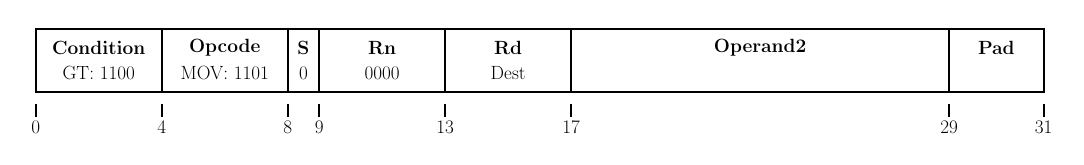
\begin{tikzpicture}[scale=0.4, every node/.style={scale=0.4}]
    % Bit fields with adjusted widths and labels for clarity
    \draw[thick] (0,0) rectangle (4,2) node[midway, yshift=0.4cm] {\textbf{\LARGE Condition}};
    \node at (2, 0.6) {\LARGE GT: 1100};
    
    \draw[thick] (4,0) rectangle (8,2) node[midway, yshift=0.4cm] {\textbf{\LARGE Opcode}};
    \node at (6, 0.6) {\LARGE MOV: 1101};
    
    \draw[thick] (8,0) rectangle (9,2) node[midway, yshift=0.4cm] {\textbf{\LARGE S}};
    \node at (8.5, 0.6) {\LARGE 0};
    
    \draw[thick] (9,0) rectangle (13,2) node[midway, yshift=0.4cm] {\textbf{\LARGE Rn}};
    \node at (11, 0.6) {\LARGE 0000};
    
    \draw[thick] (13,0) rectangle (17,2) node[midway, yshift=0.4cm] {\textbf{\LARGE Rd}};
    \node at (15, 0.6) {\LARGE Dest};
    
    \draw[thick] (17,0) rectangle (29,2) node[midway, yshift=0.4cm] {\textbf{\LARGE Operand2}};
    
    \draw[thick] (29,0) rectangle (32,2) node[midway, yshift=0.4cm] {\textbf{\LARGE Pad}};
    
    % Bit numbers
    \draw[thick] (0,-0.4) -- (0,-0.8) node[below] {\LARGE 0};
    \draw[thick] (4,-0.4) -- (4,-0.8) node[below] {\LARGE 4};
    \draw[thick] (8,-0.4) -- (8,-0.8) node[below] {\LARGE 8};
    \draw[thick] (9,-0.4) -- (9,-0.8) node[below] {\LARGE 9};
    \draw[thick] (13,-0.4) -- (13,-0.8) node[below] {\LARGE 13};
    \draw[thick] (17,-0.4) -- (17,-0.8) node[below] {\LARGE 17};
    \draw[thick] (29,-0.4) -- (29,-0.8) node[below] {\LARGE 29};
    \draw[thick] (32,-0.4) -- (32,-0.8) node[below] {\LARGE 31};

\end{tikzpicture}
\end{center}
    \begin{center}
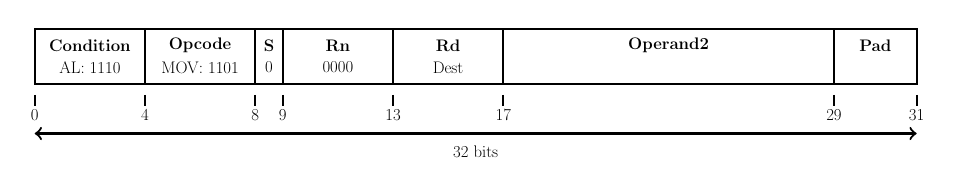
\begin{tikzpicture}[scale=0.35, every node/.style={scale=0.35}]
    % Bit fields with adjusted widths and labels for clarity
    \draw[thick] (0,0) rectangle (4,2) node[midway, yshift=0.4cm] {\textbf{\LARGE Condition}};
    \node at (2, 0.6) {\LARGE AL: 1110};
    
    \draw[thick] (4,0) rectangle (8,2) node[midway, yshift=0.4cm] {\textbf{\LARGE Opcode}};
    \node at (6, 0.6) {\LARGE MOV: 1101};
    
    \draw[thick] (8,0) rectangle (9,2) node[midway, yshift=0.4cm] {\textbf{\LARGE S}};
    \node at (8.5, 0.6) {\LARGE 0};
    
    \draw[thick] (9,0) rectangle (13,2) node[midway, yshift=0.4cm] {\textbf{\LARGE Rn}};
    \node at (11, 0.6) {\LARGE 0000};
    
    \draw[thick] (13,0) rectangle (17,2) node[midway, yshift=0.4cm] {\textbf{\LARGE Rd}};
    \node at (15, 0.6) {\LARGE Dest};
    
    \draw[thick] (17,0) rectangle (29,2) node[midway, yshift=0.4cm] {\textbf{\LARGE Operand2}};
    
    \draw[thick] (29,0) rectangle (32,2) node[midway, yshift=0.4cm] {\textbf{\LARGE Pad}};
    
    % Bit numbers
    \draw[thick] (0,-0.4) -- (0,-0.8) node[below] {\LARGE 0};
    \draw[thick] (4,-0.4) -- (4,-0.8) node[below] {\LARGE 4};
    \draw[thick] (8,-0.4) -- (8,-0.8) node[below] {\LARGE 8};
    \draw[thick] (9,-0.4) -- (9,-0.8) node[below] {\LARGE 9};
    \draw[thick] (13,-0.4) -- (13,-0.8) node[below] {\LARGE 13};
    \draw[thick] (17,-0.4) -- (17,-0.8) node[below] {\LARGE 17};
    \draw[thick] (29,-0.4) -- (29,-0.8) node[below] {\LARGE 29};
    \draw[thick] (32,-0.4) -- (32,-0.8) node[below] {\LARGE 31};

    % Arrow for full bit length label
    \draw[<->, thick] (0,-1.8) -- (32,-1.8) node[midway, below, yshift=-0.3cm] {\LARGE 32 bits};
\end{tikzpicture}
\end{center}

    \caption{Bit-level encoding of \texttt{ARMv7}'s \texttt{MOVGT} (on top) and of \texttt{MOV} (on the bottom) instructions, illustrating fields for condition codes, opcode, status bit, register operands, and operand values.}
    \label{fig:mov_encoding}
\end{figure}

In Figure \ref{fig:mov_encoding} we can observe how \texttt{MOV} and \texttt{MOVG} bit encoding only differ for the first 4 bits.
The condition field in \armvs applies to almost all instructions. In ARM’s architecture, most instructions have a 4-bit condition field. This makes non predicated instructions a particular case of predication where the condition field is set to \texttt{1110}. \\

Another architecture design that offer predication support is the Itanium \texttt{IA-64}. 
The \texttt{IA-64} has 64 predicate registers (\texttt{p0} to \texttt{63}) that allow each instruction to be conditionally executed based on specific predicate values. Each instruction can specify a predicate register, offering highly granular control over conditional execution. Thanks to this approach, entire sections of code can be totally predicated, minimizing the dependency on branch predictors.

\begin{center}
\begin{minipage}{0.5\textwidth}
\begin{lstlisting}[caption=Predicated MOV in Itanium,frame=tlrb,label={lst:itanium_predicated}]
cmp.gt p1, p0 = r0, #0
(p1) mov r1 = 10
(p0) mov r1 = 20
\end{lstlisting}
\end{minipage}
\end{center}

In Listing~\ref{lst:itanium_predicated}, it's possible to see the \texttt{IA-64} equivalent of the assembly code showed in Listing \ref{fig:branching_predication_ARM}.

\subsection{Detecting Predicable Regions}
\label{sec:detecting_pred}

Some operations are difficult to predicate. Interruption, Exceptions and System Calls have side effects that expand beyond the local execution and might trigger events that are impossible to revert. Certain Control Flow Instructions like \texttt{jmp} and \texttt{call} alter the program’s execution path, predicating this requires hardware to simulate both the taken and non-taken paths simultaneously.
Additionally, predicating large blocks results in executing many unnecessary instructions when the predicate is false. The performance penalty of executing unnecessary instructions outweighs the benefit of avoiding a branch. A set of basic block is therefore considered not predicable if it exceeds certain sizes.

% TODO do we have a definitio of Control Flow Graph somewhere? do we have a definition of Basic Block somewhere?

The discovery of predicable regions is the beginning of the \texttt{if-conversion} step. This optimization pass starts by iterating through all the basic blocks in a function's control flow graph (CFG).

\begin{figure}[H]
    \centering
    \begin{lstlisting}[style=CStyle]
/// Analyze the structure of the sub-CFG starting from the specified block.
/// Record its successors and whether it looks like an if-conversion candidate.
void IfConverter::AnalyzeBlock(
    MachineBasicBlock &MBB, std::vector<std::unique_ptr<IfcvtToken>> &Tokens) {
  // Initialize stack with the starting block.
  SmallVector<MachineBasicBlock *, 16> BBStack = {&MBB};

  while (!BBStack.empty()) {
    MachineBasicBlock *BB = BBStack.pop_back_val();
    BBInfo &BBI = BBAnalysis[BB->getNumber()];

    // Skip blocks already analyzed.
    if (BBI.IsAnalyzed) 
      continue;

    // Analyze branches and instructions in the block.
    AnalyzeBranches(BBI);
    ScanInstructions(BBI, BB->begin(), BB->end());

    // Skip blocks unsuitable for if-conversion.
    if (!BBI.IsBrAnalyzable || BBI.BrCond.empty()) {
      BBI.IsAnalyzed = true;
      continue;
    }

    // Push successors for further analysis.
    if (BBI.TrueBB && BBI.FalseBB) {
      BBStack.push_back(BBI.TrueBB);
      BBStack.push_back(BBI.FalseBB);
    }

    // Check for if-conversion patterns (e.g., diamonds, triangles).
    if (ValidDiamond(BBI)) {
      Tokens.push_back(std::make_unique<IfcvtToken>(BBI, ICDiamond));
    } else if (ValidTriangle(BBI)) {
      Tokens.push_back(std::make_unique<IfcvtToken>(BBI, ICTriangle));
    } else if (ValidSimple(BBI)) {
      Tokens.push_back(std::make_unique<IfcvtToken>(BBI, ICSimple));
    }

    BBI.IsAnalyzed = true;
  }
}
\end{lstlisting}
    \caption{Simplified version of \textit{LLVM}'s \texttt{AnalyzeBlock} implementation for \texttt{ARM} architectures.}
    \label{fig:analyze_block}
\end{figure}

For each block, the function \texttt{AnalyzeBlock} is called. A simplified version of this function is shown in Listing \ref{fig:analyze_block}.

A \textit{MachineBasicBlock} is a basic block after being translated to machine instructions.
This function analyzes the structure of a \texttt{sub-CFG} starting from a given \texttt{MachineBasicBlock}. It evaluates branches and records successors to determine if the block is suitable for \texttt{if-conversion}.
The function \texttt{AnalyzeBranches}, determines if its branches can be analyzed or reversed, and checks if it has fall-through behavior. The data collected when this function runs are then stored in the \texttt{MachineBasicBlock} struct and used later. The function \texttt{ScanInstruction} scans all the instructions in the block to determine if the block is predicable. In most cases, a block is predicable if all the instructions in the block are predicable. 
When this analysis grants that the current basic block is predicable, the function verifies if common predication patterns exists with other basic blocks. The common predication patterns are described in Subsection \ref{sec:common_predication_patterns}

The analysis, described so far, finds a set of basic blocks that are predicable and calculate the penalty for predication. if there is one.

\subsection{Compiler's Heuristics}
\label{sec:compiler_heuristics}

As already showed in Section \ref{sec:predication}, predication is versatile and can bring different advantages depending on the situation, at the same time, if applied without caution, it can result in performance degradation.
In order to decide whether to use this technique or not, modern compilers apply heuristics. These heuristics are highly architecture dependent (as Table \ref{tab:misprediction_penalty} points out). In the rest of this section, the heuristics used by the production state of the art compiler \textit{LLVM} are analyzed.

Knowing that a set of blocks, once predicated, will take a higher amount of cycles to execute is not enough to rule out predication. Two more factors have to be taken into account. The cost of misprediction and the code size.

Another crucial information that is calculated in \texttt{ScanInstruction} is whether there is an additional cost to pay when predicating the Basic Block being analyzed. The logic used to do so is reported in Listing \ref{lst:predication_cost}

\begin{figure}[H]
    \centering
    \begin{lstlisting}[style=CStyle]
BBI.NonPredSize++;
unsigned ExtraPredCost = TII->getPredicationCost(MI);
unsigned NumCycles = SchedModel.computeInstrLatency(&MI, false);
if (NumCycles > 1)
    BBI.ExtraCost += NumCycles-1;
BBI.ExtraCost2 += ExtraPredCost;
\end{lstlisting}
    \caption{Portion of code where the cost of predicating a Basic Block is calculated in \textit{LLVM}.}
    \label{lst:predication_cost}
\end{figure}

The cost of predicating a Basic Block consists of two components: architecture-dependent predication cost and instruction latency. These costs vary based on the specific instruction and the architecture. Some architectures impose a fixed cost for predicating any instruction, while others either avoid this cost entirely or apply it selectively to certain instructions. Taking as reference the \texttt{ARMv7} architecture, calls have an additional latency of 1 cycle to be predicated, while predicating any other instruction does not introduce any other cost.

\begin{figure}[H]
    \centering
    \begin{lstlisting}[style=CStyle]
bool ARMBaseInstrInfo::
isProfitableToIfCvt(MachineBasicBlock &TBB,
                    unsigned TCycles, unsigned TExtra,
                    MachineBasicBlock &FBB,
                    unsigned FCycles, unsigned FExtra,
                    BranchProbability Probability) const {
  if (!TCycles)
    return false;

  // Attempt to estimate the relative costs of predication versus branching.
  // Here we scale up each component of UnpredCost to avoid precision issue when
  // scaling TCycles/FCycles by Probability.
  const unsigned ScalingUpFactor = 1024;

  unsigned PredCost = (TCycles + FCycles + TExtra + FExtra) * ScalingUpFactor;
  unsigned UnpredCost;
  if (!Subtarget.hasBranchPredictor()) {
    // This code block contains the case where a pranch predictor
    // is not available. For the sake of brevity is not reported
  } else {
    unsigned TUnpredCost = Probability.scale(TCycles * ScalingUpFactor);
    unsigned FUnpredCost =
      Probability.getCompl().scale(FCycles * ScalingUpFactor);
    UnpredCost = TUnpredCost + FUnpredCost;
    UnpredCost += 1 * ScalingUpFactor; // The branch itself
    UnpredCost += Subtarget.getMispredictionPenalty() * ScalingUpFactor / 10;
  }

  return PredCost <= UnpredCost;
}
\end{lstlisting}
    \caption{\textit{LLVM}'s \texttt{isProfitableToIfCvt} implementation for \texttt{ARM} architectures.}
    \label{fig:predications_heuristic}
\end{figure}

\subsection{Common Predication Patterns}
\label{sec:common_predication_patterns}


\subsection{Predication Benchmarks}
\label{sec:predication_benchmark}

\newpage